% coding:utf-8

%----------------------------------------
%FOSAPMA, a LaTeX-Code for a summary of modern mathematics and physics in application.
%Copyright (C) 2013, Mario Felder

%This program is free software; you can redistribute it and/or
%modify it under the terms of the GNU General Public License
%as published by the Free Software Foundation; either version 2
%of the License, or (at your option) any later version.

%This program is distributed in the hope that it will be useful,
%but WITHOUT ANY WARRANTY; without even the implied warranty of
%MERCHANTABILITY or FITNESS FOR A PARTICULAR PURPOSE.  See the
%GNU General Public License for more details.
%----------------------------------------

\documentclass[a5paper,10pt,fleqn]{book}

\usepackage{fosapma_layout}

\title{Formelsammlung Moderne Mathematik und Physik in Anwendung}


\author{Mario Felder}
\date{\today}

\begin{document}

\maketitle

\tableofcontents
% coding:utf-8

%----------------------------------------
%FOSAPMA, a LaTeX-Code for a summary of modern mathematics and physics in application.
%Copyright (C) 2013, Mario Felder

%This program is free software; you can redistribute it and/or
%modify it under the terms of the GNU General Public License
%as published by the Free Software Foundation; either version 2
%of the License, or (at your option) any later version.

%This program is distributed in the hope that it will be useful,
%but WITHOUT ANY WARRANTY; without even the implied warranty of
%MERCHANTABILITY or FITNESS FOR A PARTICULAR PURPOSE.  See the
%GNU General Public License for more details.
%----------------------------------------

% coding:utf-8

%----------------------------------------
%FOSAPMA, a LaTeX-Code for a summary of modern mathematics and physics in application.
%Copyright (C) 2013, Mario Felder

%This program is free software; you can redistribute it and/or
%modify it under the terms of the GNU General Public License
%as published by the Free Software Foundation; either version 2
%of the License, or (at your option) any later version.

%This program is distributed in the hope that it will be useful,
%but WITHOUT ANY WARRANTY; without even the implied warranty of
%MERCHANTABILITY or FITNESS FOR A PARTICULAR PURPOSE.  See the
%GNU General Public License for more details.
%----------------------------------------

\chapter{Kerne und Teilchen}
 
\section{Coulomb Gesetz}
Coulomb-Kraft:
\[\boxed{
	F_{Coulomb} = \frac{1}{4 \pi \varepsilon_0} \frac{Q_1 \cdot Q_2}{r^2}
}\]
\\
Coulomb-Energie:
\[\boxed{
	E_{pot} = \frac{1}{4 \pi \varepsilon_0} \frac{Q_1 \cdot Q_2}{r}
}\]
\begin{footnotesize}
	$\varepsilon_0 = 8.8542 \times 10^{-12} \ \ [\frac{C}{V \cdot m}]$
\end{footnotesize}
\\


\section{Atomare Masseneinheit $u$}

\[
	\boxed{
	u = 1.660538921 \times 10^{-27}kg
	}
\]
\\
\begin{footnotesize}
Masse der Elementarteilchen:
\[
\begin{aligned}
	m_p&=1.007276466812u \\
	m_n&=1.008664916u \\
	m_e&=5.4857990946 \times 10^{-4}u
\end{aligned}
\]
\end{footnotesize}


\section{Kerngr�sse}

\[
\boxed{
	R = R_0 \cdot A^\frac13
}
\]
\begin{footnotesize}
$R_0=1.2 \times 10^{-15}m$\\
$A:$ Gesamtzahl Nukleonen, $A=Z+N$\\
\end{footnotesize}


\section{Mol}

1 mol enstpricht der \textbf{Avogadrozahl}:
\[\boxed{
	N_A=6.0221 \times 10^{23}
}\]
\\
Anzahl $mol$ eines K�rpers:
\[\boxed{
	n = \frac{N}{N_A}
}\]
\begin{footnotesize}
	$N:$ Anzahlt Teilchen in einem K�rper
\end{footnotesize}
\\
\\
Masse $m$ eines K�rpers:
\[\boxed{
	m = n \cdot m_{mol}
}\]


\section{Bindungsenergie der Kerne}

Bindungsenergie eines Atomkerns:
\[\boxed{
	E_B=\left(Z \cdot M_H + N \cdot m_n - ^A_ZM \right) \cdot c^2
}\]
\begin{footnotesize}
	$M_H:$ Masse des Wasserstoffatoms ($1.007825u$)\\
	$^A_ZM:$ Masse des neutralen Atoms\\
\end{footnotesize}
\\
mit:
\[\boxed{
	1u \cdot c^2 = 931.494061MeV
}\]
\\
Elementarladung:
\[
	1e=1.602176487 \times 10^{-19}C
\]
\\
\\
Die Atommasse pro Nukleon $\left(\frac{^A_ZM}{A}\right)$ ist ein Mass f�r die Stabilit�t des Kerns.
Je kleiner, desto st�rker die Bindung!
\[\boxed{
	\frac{-E_B}{A}=\frac{\left(Z \cdot M_H + N \cdot m_n - ^A_ZM \right) \cdot c^2}{A}
}\]


\section{Alpha Zerfall}
\begin{figure}[h!]
	\begin{center}
		\leavevmode
		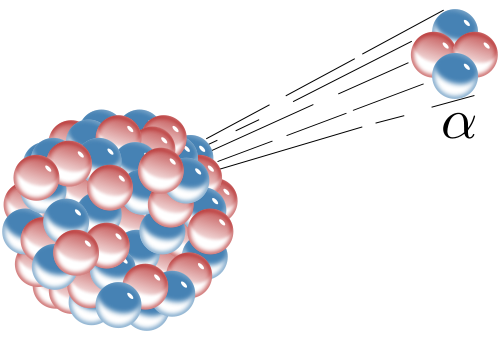
\includegraphics[scale=0.13, trim = 0mm 0mm 0mm 0mm]{../fig/alpha_decay.png}
        \caption{Alpha Zerfall}
        \label{fig:adecay}
	\end{center}
\end{figure}
~\\
Das Alpha Teilchen ist ein $^4_2He$ Kern.\\
\\
Ein Element $X$ zerf�llt:
\[\boxed{
	^A_ZX \  \rightarrow \ ^{A-4}_{Z-2}Y+\alpha+2e^-
}\]
\\
Atomare Masse von $\alpha$:
\[
	\alpha = 4.001506179125u
\]


\section{Beta Zerfall}
\begin{figure}[h!]
	\begin{center}
		\leavevmode
		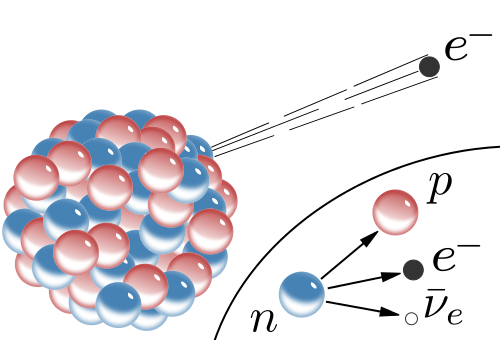
\includegraphics[scale=0.13, trim = 0mm 0mm 0mm 0mm]{../fig/beta-minus_decay.png}
        \caption{Beta-Minus Zerfall}
        \label{fig:bdecay}
	\end{center}
\end{figure}
~\\
Bei einem \textbf{Beta-Minus} Zerfall wird ein Neutron in ein Proton umgewandelt unter Aussendung eines Antineutrinos.
\[\boxed{
	n \  \rightarrow \  p + \beta^- + \overline{v_e}
}\]
\[\boxed{
	^A_ZX \  \rightarrow \  ^A_{Z+1}Y + \beta^- + \overline{v_e}
}\]
\\
Bei einem \textbf{Beta-Plus} Zerfall wird ein Proton in ein Neutron umgewandelt, unter Aussendung eines Neutrinos.
\[\boxed{
	p \  \rightarrow \  n + \beta^+ + v_e
}\]
\[\boxed{
	^A_ZX \  \rightarrow \  ^A_{Z-1}Y + \beta^+ + v_e
}\]


\section{Gamma Zerfall}
\begin{figure}[h!]
	\begin{center}
		\leavevmode
		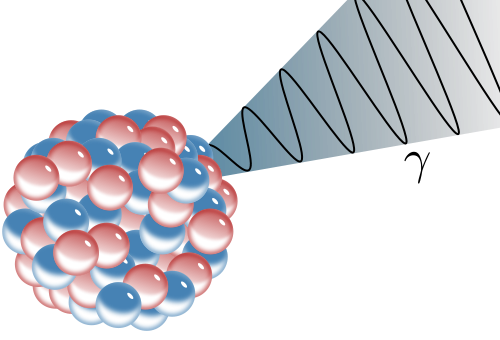
\includegraphics[scale=0.13, trim = 0mm 0mm 0mm 0mm]{../fig/gamma_decay.png}
        \caption{Beta-Minus Zerfall}
        \label{fig:bdecay}
	\end{center}
\end{figure}
~\\
Beim Gamma Zerfall befindet sich das Atom in einem angeregten Zustand und sendet dan ein hochenergetisches Photon ($\gamma$) aus.\\
\\
Es ensteht kein neues Element, sondern der Kern f�llt nur in einen energetisch tieferen Zustand.\\
\\
\[\boxed{
	E_{Photon}=h \cdot f
}\]
\\
Plancksche Konstante:
\[
	h=6.6261 \times 10^{-34}J \cdot s
\]


\section{Elektromangetisches Spektrum}
F�r jede elektromagnetische Welle gelten folgende Gleichungen:
\[\boxed{
\begin{aligned}
	c &= f \cdot \lambda \\
	p_\gamma &= \frac{h}{\lambda} \\
	E_\gamma &= h \cdot f = h \cdot \frac{c}{\lambda} = p_\gamma \cdot c
\end{aligned}
}\]
\begin{footnotesize}
	$f:$ Frequenz \\
	$\lambda:$ Wellenl�nge \\
	$p_\gamma:$ Impuls \\
	$E_\gamma:$ Energie des Photons\\
	\\
	$c = 299'792'458 \frac{m}{s}$\\
	$h = 6.626069 \times 10^{-34} J \cdot s$
\end{footnotesize}


\section{Halbwertszeit und Aktivit�t}
Radioaktives Zerfallsgesetz:
\[\boxed{
	N(t)=N_0 \cdot \ex{-\beta \cdot t}
}\]
\begin{footnotesize}
	$\beta:$ Zerfallskonstante
\end{footnotesize}
\\
\\
Halbwertszeit:
\[\boxed{
	T_{\frac12} = \frac{\ln{2}}{\beta} = \ln{2} \cdot \tau
}\]
\begin{footnotesize}
	$\tau:$ Zerfallszeit ($\frac1\beta$)
\end{footnotesize}
\\
\\
Aktivit�t:
\[\boxed{
	A=\left| \frac{\di N}{\di t} \right| = \beta \cdot N = \frac{N}{\tau}
}\]
~\\
\begin{footnotesize}
	Becquerel: $1 Bq = 1$ Zerfall/Sekunde\\
	Curie: $1 Ci = 3.70 \times 10^{10}Bq$
\end{footnotesize}


\section{$^{14}C$-Datierung}
Alles Lebendige enth�lt $^{14}C$. Das $^{14}C$ entsteht kontinuierlich durch kosmische Bestrahlung.\\
\\
Das nat�rliche Verh�ltnis:
\[\boxed{
	\frac{^{14}C}{^{12}C} = 1.3 \times 10^{-12}
}\]
\\
\\
Halbwertszeit von $^{14}C$:
\[\boxed{
	T_{\frac12} = 5730 \mathrm{\text{ Jahre}}
}\]
\\


\section{Strahlendosis}
Die absorbierte Energie pro kg lebendes Gewege nennt man \textbf{Energiedosis} D:
\[\boxed{
	[D] = 1 Gray = 1Gy = 1 \frac{J}{kg} = 100rad
}\]
\\
Der biologische Effekt wird beschrieben durch die \textbf{�quivalentdosis} H:
\[\boxed{
	[H] = 1 Sievert = 1 Sv = 100rem
}\]
\\
Bewertugnsfaktor q:
\[\boxed{
	H = D \cdot q
}\]
\begin{footnotesize}
	$[q] = \frac{Sv}{Gy}$
\end{footnotesize}
\\
\\
\begin{tabular}{|l|c|}
	\hline
	Strahlung		&	$q$ [$\frac{Sv}{Gy}$]	\\
	\hline
	\rowcolor{white}$\gamma$		&	1				\\
	\rowcolor{lgray}$\beta$		&	1 - 1.5			\\
	\rowcolor{white}langsame $n$	&	3				\\
	\rowcolor{lgray}$n$ (0.02 - 0.1MeV)&	5 - 8				\\
	\rowcolor{white}schnelle $n$ und $p$&10				\\
	\rowcolor{lgray}$\alpha$		&	20				\\
	\rowcolor{white}schwere Kerne 	&	20				\\
	\hline
\end{tabular}\\
\\
\\
Die Frei werdende Energie einer Nuklearexplosin wird mit dem Energie�quivalent des Sprengstoffs TNT verglichen.
\[\boxed{
	1kT = 4.184 \times 10^{12} J
}\]
\\


\section{Wenig Zerf�lle - Poisson Statistik}
Der radioaktive Zerfall eines Kerns ist \textbf{echt zuf�llig}
\[\boxed{
	p(x) = \frac{m^x \cdot \ex{-m}}{x!} = \frac{m^x \cdot e^{-m}}{\int_0^\infty \left(t^x \cdot \ex{-t} \right) \di t}
}\]
\begin{footnotesize}
	$p(x)$ ist die Wahrscheinlichkeitsdichte f�r den Wert $x$ bei einem Mittelwert von $m$.
\end{footnotesize}
\\


\section{Viele Zerf�lle - Gauss Statistik}
F�r lange Messzeiten, d.h. gross Mittelwerte geht die Poisson Verteilung in die Gaussverteilung �ber:
\[\boxed{
	p(x) = \frac1{\sqrt{2\pi \cdot m}} \cdot \ex{\frac{-\left(x - m\right)^2}{2m}}
}\]
\\
Standard Abweichung:
\[
	\sigma = \sqrt{m}
\]
\\


\section{Nukleare Reationen}
Zwei Kerne $A$ und $B$ verwandeln sich in einem Prozess zu Kernen $C$ und $D$.
Die \textbf{Reaktionsenergie} Q berechnet sich:
\[\boxed{
	Q = \left( M_A + M_B -M_C -M_D \right) \cdot c^2
}\]


\subsection{exotherm}
Ist Q positiv, wird die gesamte Masse kleiner und die kinetische Restenergie gr�sser.

\subsection{endotherm}
Ist Q negativ, wird die gesamte Masse gr��ser und die kinetische Energie kleiner.\\
Eine endotherme Reaktion ist nur m�glich, wenn die gewonnene Masse in Form kinetischer Energie vorhanden ist.
Dabei entspricht der Betrag von Q gleich der kinetischen Energie im Schwepunktsystem:
\[
	\left|Q\right| = Q_{cm}
\]
\\
Wenn der einte K�rper in Ruhe ist, muss sich der andere mit folgender Energie ann�hern:
\[\boxed{
	E_{kin,a}=\frac{M_b + M_a}{M_b} \cdot Q_{cm}
}\]
\\

\section{Kernspaltung}
Durch Neutronenbeschuss eines Kerns bei gelegentlichem Beta Zerfall kann seine Massenzahl (Anzahl Nukleonen) um bis zu 25 erh�ht werden.\\
Der Neutronenbeschuss von $^{238}U$ (99.3\%) oder $^{235}U$ (0.7\%) f�hrt zu deren Spaltung in kleinere Fragmente.\\
Nicht das $^{235}U$ zerf�llt, sondern das hoch angeregte $^{235}U^*$.
Dies gem�ss zwei typischen Varianten:
\[\boxed{
	^{235}_{92}U + ^1_0n \ \rightarrow\ ^{235}_{92}U^* \ \rightarrow\ ^{144}_{56}Ba + ^{89}_{36}Kr + 3 \cdot ^1_0n
}\]
\[\boxed{
	^{235}_{92}U + ^1_0n \ \rightarrow\ ^{235}_{92}U^* \ \rightarrow\ ^{140}_{54}Xe + ^{94}_{38}Sr + 2 \cdot ^1_0n
}\]
\\
\\
\\
Der wichtige Unterschied:\\
\fbox{\parbox{\linewidth}{
	\textbf{Radioaktivit�t:} \underline{Spontaner} Zerfall instabiler Isotop wie $^{14}C$. Der Zerfall erfolgt echt zuf�llig. Die H�lfte der radioaktiven Kerne ist nach der Halbwertszeit $T_{\frac12}$ zerfallen.\\
	\\
	\textbf{Kernreaktion:} \underline{Erzwungene} Umwandlung der Kerne, beispielsweise durch Beschuss mit Neutronen. Die neu entstehenden Kerne k�nnen allerdings radioaktiv sein und spontan weiter zerfallen.
}}

\section{Aktivierungsenergie}
Zwei Kerne m�ssen sich f�r die Fusion so weit ann�hern, dass die starke Kernkraft wirksam wird, typischerweise auf etwa $2 \times 10^{-15}m$.\\
\\
Die durchschnittliche kinetische Energie von Teilchen bei Temperatur T:
\[
	E_{kin} = \frac{3}{2} k_B \cdot T
\]
\begin{footnotesize}
	$k_B = 1.3806488 \times 10^{-23}\ \frac{J}{K}$
\end{footnotesize}
   
% coding:utf-8

%----------------------------------------
%FOSAPMA, a LaTeX-Code for a summary of modern mathematics and physics in application.
%Copyright (C) 2013, Mario Felder

%This program is free software; you can redistribute it and/or
%modify it under the terms of the GNU General Public License
%as published by the Free Software Foundation; either version 2
%of the License, or (at your option) any later version.

%This program is distributed in the hope that it will be useful,
%but WITHOUT ANY WARRANTY; without even the implied warranty of
%MERCHANTABILITY or FITNESS FOR A PARTICULAR PURPOSE.  See the
%GNU General Public License for more details.
%----------------------------------------

\chapter{Relativit�tstheorie}

\fbox{\parbox{\linewidth}{
	Die spezielle Relativit�tstheorie basiert auf zwei einfachen und intuitiven Postulaten:
	\begin{enumerate}[label=\textbf{\Roman*.}]
		\item Alle physikalischen Gesetzte gelten gleichermassen in jedem Inertialsystem
		\item Die Vakuumlichtgeschwindigkeit ist konstant und exakt \textbf{$c=299'792'458 \frac{m}{s}$} in allen Inertialsystemen.
\end{enumerate}
}}

\newpage
\section{Bestimmung der Lichtgeschwindigkeit}

Maxwell konnte aus seinen vier Gleichungen die Wellengleichung f�r elektromagnetische Wellen ableiten. Daraus ergibt sich die Lichtgeschwindigkeit als:
\[\boxed{
	c = \frac{1}{\sqrt{\varepsilon_0 \cdot \mu_0}}
}\]
\\
\begin{footnotesize}
	die elektrische Feldkonstante $\varepsilon_0 = 8.8542 \times 10^{-12} \frac{As}{Vm}$\\
	die magnetische Feldkonstante $\mu_0 = 4 \cdot \pi \times 10^{-7} \frac{Vs}{Am}$ 
\end{footnotesize}
\\


\section{Zeitdilatation $\gamma$}
Ein Beobachter im System $S$, misst eine andere Zeit $\Delta t$ f�r ein Ereignis im bewegtem System $S'$:
\[\boxed{
	\Delta t = \gamma \cdot \Delta t_0
}\]

\[
	\beta = \frac{u}{c} \\ \gamma = \frac{1}{\sqrt{1-\frac{u^2}{c^2}}} = \frac{1}{\sqrt{1-\beta^2}}
\]

\subsection{Eigenzeit $\Delta t_0$}
Es existiert nur ein Bezugssystem, in dem eine Uhr in Ruhe ist. ALle anderen Bezugssysteme sind dazu bewegt und werden diese Uhr nachgehen sehen. \textbf{Zeitintervalle am gleichen Ort sind die k�rzesten.}
\\


\section{L�ngenkontraktion $\frac{1}{\gamma}$}
Ebenfalls misst ein Beobachter im System $S'$ eine andere L�nge $L'$ f�r eine L�nge $L_0$ parallel zur Bewegung im relativ bewegtem System $S$:
\[\boxed{
	L = L_0 \cdot \sqrt{1 - \frac{u^2}{c^2}} = \frac{L_0}{\gamma}
}\]

\subsection{Eigenl�nge $L_0$}
In allen zu $S'$ bewegten Bezugssystemen messen die Beobachter eine kleinere L�nge $L$, und zwar umso kleiner, je gr�sser die Relativgeschwindigkeit $u$ ist.
\\


\section{Formverzerrung}
Durch die L�ngenkontraktion werden Formen verzerrt. Ein Quadrat im System $S'$ wird zu einem Parallelogramm im System $S$. Der Beobachter im System $S$ sieht den Winkel zur Bewegungsrichtung als:
\[\boxed{
	\theta = \arctan \left( \gamma \cdot \frac{\sin \theta '}{\cos \theta '} \right)
}\]
\\


\section{Lorentz Transformationen}
Koordinaten:
\[\boxed{
	\begin{aligned}
		x &= \frac{x'+ut'}{\sqrt{1-\frac{u^2}{c^2}}} = \gamma (x' + ut') \\
		y &= y' \\
		z &= z' \\
		t &= \frac{t' + \frac{ux'}{c^2}}{\sqrt{1-\frac{u^2}{c^2}}} = \gamma (t' + \frac{ux'}{c^2}) 
	\end{aligned}
}\]
\\
Geschwindigkeiten:
\[\boxed{
	\begin{aligned}
		v_x &= \frac{v_x'+u}{1+\frac{u \cdot v_x'}{c^2}} \\
		v_y &= \frac{v_y' \cdot \sqrt{1-\frac{u^2}{c^2}}}{1+\frac{u \cdot v_x'}{c^2}} \\
		v_z &= \frac{v_z' \cdot \sqrt{1-\frac{u^2}{c^2}}}{1+\frac{u \cdot v_x'}{c^2}}  
	\end{aligned}
}\]
\\
Kr�fte:
\[\boxed{
	\begin{aligned}
		F_x &= \frac{F_x' + \frac{u}{c^2} \left( \vec{F}' \cdot \vec{v}' \right)}{1+\frac{u \cdot v_x'}{c^2}} \\
		F_y &= \frac{F_y' \cdot \sqrt{1-\frac{u^2}{c^2}}}{1+\frac{u \cdot v_x'}{c^2}} \\
		F_z &= \frac{F_z' \cdot \sqrt{1-\frac{u^2}{c^2}}}{1+\frac{u \cdot v_x'}{c^2}}  
	\end{aligned}	
}\]
\\
Die Bewegungsrichtung ist die $x$-Achse. Alle gestrichenen Gr�ssen sind gemessen in $S'$. $u$ ist die Relativgeschwindigkeit der beiden Systeme. $u$ ist positiv f�r $S$, und negativ f�r $S'$. Die Beziehungen lauten genau gleich, nur erh�lt $u$ ein negatives Vorzeichen!
\\
\\
\\
W�hlt man statt der Zeit $t$ die Lichtl�nge $ct$ werden die Lorentz Transformationen:
\[
	x = \gamma \left( x' + \frac{u}{c}ct' \right)	\\ ct = \gamma \left( ct' + \frac{u}{c} x' \right)
\]
\\

\subsection{Relativistischer Impuls}
Relativistischer Impuls:
\[\boxed{
	\vec{p} = \frac{m_0 \cdot \vec{v}}{\sqrt{1-\frac{v^2}{c^2}}} = \gamma m_0 \vec{v}
}\]
\\
daraus kann eine relativistische Masse definiert werden:
\[\boxed{
	m_{rel} = \frac{m_0}{\sqrt{1-\frac{v^2}{c^2}}} = \gamma m_0
}\]
\\

\subsection{Zweites Newtonsches Gesetz}
Anhand der urspr�nglichen Formulierung Newtons:
\[\boxed{
	\vec{F} = \frac{\di \vec{p}}{\di t} = \frac{\di}{\di t} \gamma m_0 \vec{v}
}\]
\\
\\
Fall \textbf{(1)}: $\vec{F}$ und $\vec{v}$ sind parallel
\[\boxed{
	\vec{F}_{||} = \frac{m_0}{ \left( 1-\frac{v^2}{c^2} \right)^{\frac32}} \cdot \vec{a}_{||} = \gamma^3 m_0 \vec{a}_{||}
}\]
\\
Fall \textbf{(2)}: $\vec{F}$ und $\vec{v}$ sind senkrecht ($v^2 = $konst)
\[\boxed{
	\vec{F}_{\bot} = \frac{m_0}{ \sqrt{1-\frac{v^2}{c^2}}} \cdot \vec{a}_{\bot} = \gamma m_0 \vec{a}_{\bot}
}\]
\\
\begin{footnotesize}
	Aus \textbf{(1)} und \textbf{(2)} folgt, dass bei hohen Geschwindigkeiten Beschleunigung und Kraft nicht mehr parallel sind!\\
	$\frac{F_{\shortparallel}}{F_{\bot}} = \gamma^2 \frac{a_{\shortparallel}}{a_{\bot}}$
\end{footnotesize}
\\

\subsection{Masse $=$ Energie}
Relativistische kinetische Energie:
\[\boxed{
	E_{kin} = \frac{m_0 \cdot c^2}{\sqrt{1-\frac{v^2}{c^2}}} - m_0 \cdot c^2 = (\gamma - 1) \cdot m_0 \cdot c^2
}\]
\\
Gesamte Energie:
\[\boxed{
	E = E_{kin} + m_0 \cdot c^2 = \gamma m_0 \cdot c^2 = m_{rel} \cdot c^2
}\]
\\
\begin{footnotesize}
	$m_0 \cdot c^2$: Ruheenergie \\
	$m_0$ ist die Ruhemasse aus Tabellen
\end{footnotesize}
\\

\subsection{Invariante Gr�ssen}
Alternativ kann auch geschrieben werden:
\[
	E^2 = \left( m_0 \cdot c^2 \right)^2 + (pc)^2
\]
\\
\begin{footnotesize}
	Diese Gleichung gilt auch f�r masselose Teilchen, beispielsweise f�r Photonen: $E_{Photon} = 0 + pc = \frac{h}{\lambda} c = h \cdot f$
\end{footnotesize}
\\
\\
Invariante Form der Ruheenergie:
\[\boxed{
	m_0 \cdot c^2 = \sqrt{E^2 - (pc)^2}
}\]
\\
Invariante Form des Raum-Zeit Intervalls:
\[\boxed{
	\Delta s^2 = (c \cdot \Delta t)^2 - \left[ \Delta x^2 + \Delta y^2 + \Delta z^2 \right] 
	\begin{aligned}
		&= (c \cdot \Delta t_0)^2 \\
		&= -{L_0}^2
	\end{aligned}
}\]
\\
\begin{footnotesize}
	$\Delta s^2 = -{L_0}^2$ = \textbf{raumartig} \\
	Zeitintervall ist null, beide Ereignisse finden gleichzeitig statt.\\
	\\
	$\Delta s^2 = (c \Delta t_0)^2$ = \textbf{zeitartig} \\
	Ereignise finden am gleichen Ort, aber zu unterschiedlichen Zeiten statt.
\end{footnotesize}



\section{Minkowski Diagramm}

Mit Hilfe eines Minkowski Diagramms k�nnen Zusammenh�nge von zwei Systemen $S$ und $S'$ einfach ausgelesen werden.\\
F�r jedes Ereignis k�nnen Ort und Zeit f�r das jeweilige System zugeordnet werden.
\begin{center}
	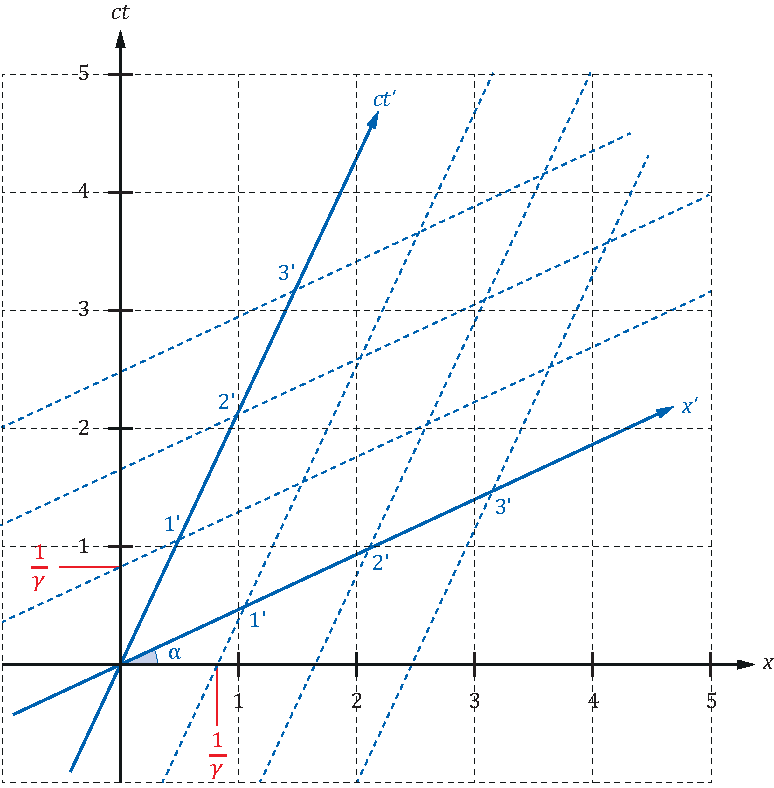
\includegraphics[scale = 0.75]{../fig/minkowski_diagramm}
\end{center}
~\\
Der Winkel $\alpha$ ergibt sich aus:
\[\boxed{
	\tan \alpha = \frac{u}{c}
}\]
\\


\section{Relativit�t der Elektrodynamik}

In Bezug auf die Relativ-Geschwindigkeit $u$ wird zwischen parallelen und senkrechten Feldkomponenten unterschieden.

\[\boxed{
\begin{matrix}
	E_{||}' = E_{||}	&&	B_{||} = B_{||}	\\
	E_{\bot}' = \gamma \left( \vec{E} + \vec{u} \times \vec{B} \right)_{\bot}	&& B_{\bot}' = \gamma \left( \vec{B} - \frac{\vec{u} \times \vec{E}}{c^2} \right)_{\bot}	
\end{matrix}
}\]
\\


\section{Dopplereffekt von elektro-magn. Wellen}
Da elektro-magnetische Wellen kein Tr�germedium ben�tigen, muss nicht wie beim Schall speziell zwischen der Bewegung der Quelle ud des Beobachters unterschieden werden.
\[\boxed{
\begin{matrix}
	f = \sqrt{\frac{c+u}{c-u}} \cdot f_0' && \  && \frac{f-f_0'}{f_0'} = \frac{\Delta f}{f_0'}
\end{matrix}
}\]
\\
\begin{footnotesize}
	$u$ positiv: Quelle bewegt sich auf den Beobachter zu \\
	$u$ negativ: Quelle bewegt sich vom Beobachter weg
\end{footnotesize}
\\


\section{Headlight Effekt - Beaming Effekt}
Die Lichtgeschwindigkeit ist in jedem Bezugssystem gleich. Nicht gleich ist aber die Richtung der Strahlung.\\
Eine isotrope Quelle bewege sich mit der Geschwindigkeit $u$ bez�glich des Laborsystems $S$. Im Laborsystem $S$ strahlt die Quelle  vor allem in die Vorw�rtsrichtung.
\begin{center}
	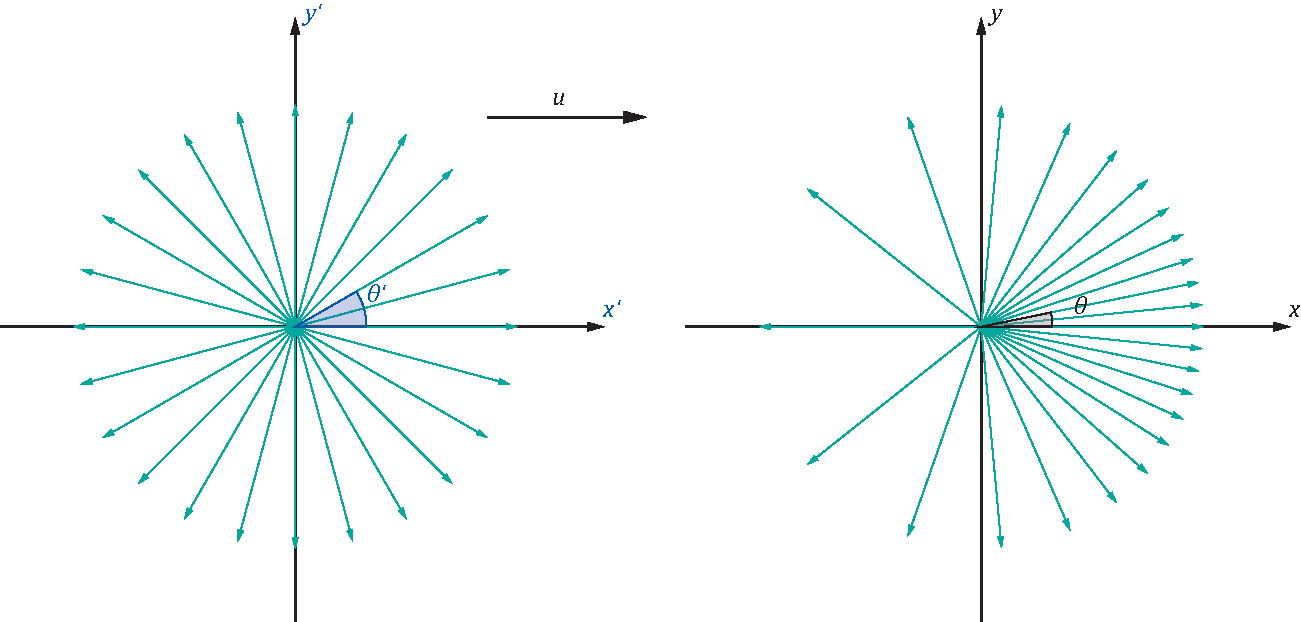
\includegraphics[scale = 0.4]{../fig/beaming_effekt}
\end{center}

\[\boxed{
	\cos \theta = \frac{\cos \theta' + \frac{u}{c}}{1 + \frac{u}{c} \cos \theta'}
}\]
\\
\\
�hnliches gilt f�r die anderen trigonometrischen Funktionen:
\[\begin{matrix}
	\sin \theta = \frac{\sin \theta '}{\gamma \left( 1 + \frac{u}{c} \cos \theta ' \right)} && 
	\tan \theta = \frac{\sin \theta '}{\gamma \left( \cos \theta ' + \frac{u}{c} \right) }
\end{matrix}\]
\\


\subsection{Aberration des Lichts}
\begin{center}
	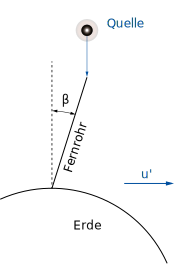
\includegraphics[scale = 0.5]{../fig/aberration}
\end{center}
Aberrationswinkel:
\[\boxed{
	\tan \beta = \frac{v_x}{v_y} = \frac{\frac{u}{c}}{\sqrt{1-\frac{u^2}{c^2}}}
}\]
\\
\textit{Achtung:} Der Winkel $\beta$ ist ein anderer als $\theta$!\\
$\tan \beta = \frac1{\tan \theta} = \cot \theta$
\\


\section{Strahlung beschleunigter Elektronen}

Pointing-Vektor in Richtung Beobachter:
\[\boxed{
	S(r)=\frac{\di P}{\di A} = \frac{q_e^2 a^2 \sin^2 \varphi}{\left( 4 \pi \right)^2 \varepsilon_0 c^3 r^2}\ \ \left[ \frac{W}{m^2} \right]
}\]
\begin{center}
	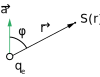
\includegraphics[scale = 0.75]{../fig/pointing_vector}
\end{center}
~\\
\begin{footnotesize}
	$q_e$: Elementarladung $1.6 \times 10^{-19}C$ \\
	$a$: Beschleunigung des Elektrons \\
	$\varphi$: Beobachtungsrichtung \\
	$r$: Abstand des Beobachters zum Elektron
\end{footnotesize}
\\
\\
Abstrahlung pro Raumwinkel $\di \Omega$:
\[\boxed{
	\frac{\di P}{\di \Omega} = \frac{q_e^2 a^2 \sin^2 \varphi}{\left( 4 \pi \right)^2 \varepsilon_0 c^3}\ \ \left[ \frac{W}{sr} \right]	
}\]
\\


\subsection{Synchrotron Strahlung}

In einem Synchrotron bewegen sich geladene Teilchen mit nahezu Lichtgeschwindigkeit im Kreis herum. Die Beschleunigung $a$ bei gleichbleibender Geschwindigkeit zeigt zum Kreismittelpunkt.
\\
\begin{center}
	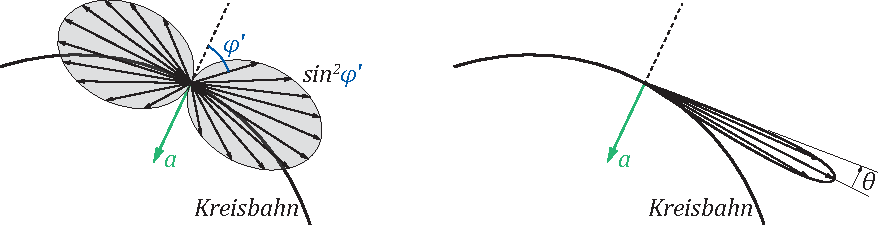
\includegraphics[scale = 0.7]{../fig/synchrotron}
\end{center}
~\\
Im System $S'$ strahlt die Quelle ringf�rmig ab. Im Laborsystem $S$ strahlt die Quelle vorw�rts ab, die charakteristische Synchrotron-Strahlung.
\[
	\tan \theta = \frac{\sin \theta '}{\gamma \left( \cos \theta ' + \frac{u}{c} \right)}
\]


\end{document}

